\documentclass[11pt,a4paper]{article}
\usepackage[margin=1in]{geometry}
\usepackage{amsmath,amssymb}
\usepackage{graphicx}
\usepackage{booktabs}
\usepackage{longtable}
\usepackage{array}
\usepackage{siunitx}
\usepackage{hyperref}
\usepackage{float}
\usepackage{listings}
\usepackage{enumitem}
\usepackage{fancyhdr}
\usepackage{setspace}
\usepackage{caption}
\usepackage{subcaption}
\usepackage{titlesec}

\title{Real-Time GNC Loop Under Emulation}
\author{Rakshita Basagoudar\\Electronics and Communication Engineering\\GM Institute of Technology, Davangere}
\date{October 2026}

\begin{document}
\onehalfspacing
\maketitle
\tableofcontents
\listoffigures
\listoftables
\newpage
\tableofcontents
\newpage
\section{Abstract}
This project develops and verifies a reproducible real-time Guidance, Navigation and Control (GNC) software loop for a representative spacecraft attitude-control application under ARM Cortex-M4 emulation. The implementation follows a Python reference model, a C embedded controller, FreeRTOS task integration, and Renode-based execution. The principal controller is a proportional-derivative law with reaction-wheel torque saturation. The work evaluates functional correctness, real-time execution, timing, jitter, robustness, cross-code agreement, convergence, published-reference comparison, and reproducibility.

The deterministic cross-code verification produced exact agreement between the Python reference and the embedded C implementation for the test input, with torque values of -0.010000, +0.007000, and -0.003300 N.m. The analytical actuator limit of +/-0.010 N.m per axis was also verified. A dedicated controller benchmark produced a maximum observed execution time of 7.288 microseconds at 125 MIPS. For a 10 ms GNC period, the corresponding observed timing margin is 9.992712 ms. Week 11 measured a 10 ms activation period with zero measured peak-to-peak jitter at the available 1 ms timer resolution.

The four-way verification campaign covers analytical limits, published data, cross-code verification, and convergence. Analytical and cross-code checks are directly verified. The convergence study is verified at the reported output precision, with the limitation that it does not independently prove the internal adaptive RK45 truncation convergence. Published-data verification remains partial because the original numerical target-tracking time series from the published ARAPAIMA STK simulation were unavailable. The published 0.35 arcmin benchmark was identified and Figure 5.4 was digitized, producing a mean of 0.3911 arcmin and a relative difference of 11.74 percent. This is reported as a qualified comparison rather than a reproduction of the original simulation data.

The project also documents unsuccessful and limited measurements. An early timing attempt ended in an INVSTATE UsageFault and was excluded from timing claims. Several legacy Renode scripts retain machine-specific absolute paths, while a clean relative-path Week 9 reproduction script was created and verified. The final result therefore distinguishes verified evidence, qualified evidence, and remaining gaps rather than presenting unsupported results as successful reproductions.

\section{Introduction}
Small spacecraft require attitude-control software that is not only mathematically correct but also executable under realistic embedded timing constraints. The project therefore treats the GNC controller as both a control-law implementation and a real-time embedded software artifact. The central objective is to establish an evidence-driven and partially reproducible path from a Python reference model to C code running on an emulated ARM Cortex-M4 target with FreeRTOS scheduling and Renode execution. This work was carried out as part of the EduRankAI Electronics Engineering Internship under the VISVAMBHARA technical task assignment.

\textbf{Project Contribution.} The work covered the embedded C controller implementation, FreeRTOS task integration, Renode-based Cortex-M4 execution, timing measurements, Python/C cross-code verification, robustness analysis, and reproducibility documentation.

The selected application is spacecraft attitude control using a proportional-derivative controller and reaction-wheel actuation. The implementation uses a quaternion-based spacecraft state representation together with angular-rate and wheel-momentum states. The controller output is constrained by the specified reaction-wheel torque limit. This provides a compact but meaningful test case for examining numerical behaviour, embedded implementation, task scheduling, timing, and robustness within one reproducible workflow.\par

A major objective of the work is to distinguish measured evidence from assumptions. Execution-time measurements are reported as observed measurements rather than formal worst-case execution-time proofs. Similarly, the published-reference comparison is explicitly qualified because the original numerical time series used to generate the published benchmark was not available. Failed experiments, including the initial INVSTATE timing failure, are retained as part of the verification record because they identify limitations of the implementation and measurement process.\par

The remainder of this report presents the system model, implementation, verification methodology, timing and jitter measurements, cross-domain integration, robustness analysis, published-reference comparison, reproducibility assessment, limitations, and recommendations for further work.\par

\section{Project Requirements and Verification Strategy}

The project was developed against the weekly technical and documentation requirements defined in the task assignment. The work progressed from an analytical model and reference implementation to an embedded artifact, timing measurements, validation, integration, robustness testing, and final reproducibility documentation. The verification strategy was designed to provide independent evidence through analytical limits, comparison with a published result, cross-code agreement, and numerical convergence.\par

The principal requirements addressed in this report are:
\begin{enumerate}[leftmargin=*]
\item establish a documented analytical model and control-law implementation;
\item produce a working embedded C artifact capable of executing the controller;
\item integrate the controller into a FreeRTOS-based task structure and execute it under Cortex-M4 emulation;
\item measure controller execution behaviour and the periodic activation interval;
\item verify agreement between the Python reference implementation and embedded C implementation;
\item perform convergence, parameter-sensitivity, Monte Carlo, and edge-case studies;
\item compare the work with an identified published spacecraft attitude-control result;
\item exchange a real software artifact between the GNC model and embedded-software side and verify the resulting interface; and
\item document failures, limitations, reproduction steps, and remaining gaps without presenting unsupported results as successful verification.
\end{enumerate}

The resulting evidence is classified into three categories: \textbf{verified}, where the available experiment directly supports the claim; \textbf{verified with qualification}, where the evidence supports the stated claim but has a defined measurement or interpretation limitation; and \textbf{partial/qualified}, where the requested verification could not be fully reproduced because required external data were unavailable. This classification is used throughout the report to maintain traceability between requirements and evidence.

\section{System Model and Control Law}

\subsection{Spacecraft and Reaction-Wheel Model}

The reference spacecraft is the VESPER-SAT-6U representative model used by the project implementation. The default spacecraft inertia matrix is diagonal, with principal moments of 0.05, 0.04, and 0.06 kg m2. The model uses three reaction-wheel axes, with a maximum wheel torque magnitude of 0.010 N m and a maximum stored momentum magnitude of 0.100 N m s.

The state representation uses the quaternion convention q = [qx, qy, qz, qw]T, with the scalar component as the final element. The angular velocity vector is represented by omega = [omega_x, omega_y, omega_z]T. The complete model additionally tracks the three reaction-wheel momentum states.\subsection{Proportional-Derivative Control Law}

The embedded controller implements a proportional-derivative control law using the attitude-error vector and body angular-rate vector. The raw commanded torque is defined by the proportional and derivative gains used throughout the verified implementation.

\begin{equation}
\tau_{\mathrm{raw}}=-K_p q_{\mathrm{err}}-K_d\omega.
\end{equation}

The gains used throughout the verified implementation are: 
\begin{equation}
K_p=0.008,\qquad K_d=0.05.
\end{equation}


For each axis, the analytical torque bound is:
\begin{equation}
|\tau_{\mathrm{raw},i}|\leq K_p|q_{\mathrm{err},i}|+K_d|\omega_i|.
\end{equation}

The final commanded torque is clipped to the reaction-wheel limit:
\begin{equation}
\tau_i=\operatorname{clip}(\tau_{\mathrm{raw},i},-0.010,+0.010)\ {\rm N\,m}.
\end{equation}

This saturation is part of the embedded controller implementation and is included in the analytical and functional verification.


\subsection{Analytical Verification Case}

A deterministic test case was used to verify the controller calculation and actuator limit. The input vectors are:
\begin{equation}
q_{\mathrm{err}}=[0.5,-0.25,0.1]^T,\qquad \omega=[0.2,-0.1,0.05]^T.
\end{equation}

The resulting raw torque is [-0.014, 0.007, -0.0033] N m. After applying the actuator limit, the expected commanded torque is [-0.010, 0.007, -0.0033] N m. The first axis therefore exercises the torque saturation while the other two axes remain unsaturated.


\subsection{Dynamics and Numerical Reference}

The Python reference model propagates quaternion attitude, body angular rate, and reaction-wheel momentum. The rotational dynamics include the rigid-body gyroscopic term together with the applied reaction-wheel and external torques. Quaternion kinematics are computed from the body angular-rate vector, while wheel momentum evolves according to the commanded wheel torque.

The principal reference simulations use the Python numerical environment established during the project and an adaptive SciPy integration method. The later convergence study varies the requested output step and compares the resulting final attitude. Because the solver remains adaptive internally, this convergence evidence is treated as an output-level numerical check rather than a formal proof of internal RK45 truncation-error convergence.


\section{Reference Simulation and Baseline Results}

The LQR implementation uses the six-state vector $x=[\delta q_x,\delta q_y,\delta q_z,\omega_x,\omega_y,\omega_z]^T$, with the attitude-error vector obtained from the quaternion error. The linearized model is defined by $A_{1:3,4:6}=0.5I_3$ and $B_{4:6,:}=I^{-1}$, using the spacecraft inertia $I=\operatorname{diag}(0.05,0.04,0.06)\,\mathrm{kg\,m^2}$. The default weighting matrices are $Q=\operatorname{diag}(5,5,5,0.5,0.5,0.5)$ and $R=\operatorname{diag}(50,50,50)$. The continuous-time algebraic Riccati equation is solved using SciPy, and the feedback gain is computed as $K=R^{-1}B^TP$. For the project parameters, the resulting gain matrix is $K=\begin{bmatrix}0.31622777&0&0&0.16065923&0&0\\0&0.31622777&0&0&0.15049621&0\\0&0&0.31622777&0&0&0.17021653\end{bmatrix}$. The commanded torque is $\tau=-Kx$ and is clipped to the reaction-wheel limit of $\pm0.010\,\mathrm{N\,m}$. If the Riccati solution fails, the implementation contains a documented PD-equivalent fallback gain; the reported LQR scenarios use the normal LQR controller path.

The Python reference model was used to establish the baseline behaviour against which the embedded implementation was evaluated. Four representative scenarios were retained: free drift, 30 degree rest-to-rest attitude control using PD and LQR controllers, and a 45 degree yaw-slew case using PD and LQR controllers.

\subsection{Free-Drift Case}

For the 600 s free-drift simulation, the final angular-rate magnitude was 0.0436 deg/s. The final roll angle was -31.479 degrees, while the final pitch and yaw angles were approximately zero. The maximum Euler-angle error was 31.479 degrees and no actuator saturation occurred. This case provides a useful uncontrolled-dynamics baseline.

\subsection{Rest-to-Rest and Yaw-Slew Cases}

For the 30 degree rest-to-rest case over 200 s, the PD controller reached an approximately zero final attitude error with a maximum Euler-angle error of 30 degrees and 1.8 percent actuator saturation. The corresponding LQR case also reached approximately zero final attitude error but exhibited 14.3 percent saturation.

For the 45 degree yaw-slew case over 300 s, the PD controller reached approximately -45 degrees final yaw with 3.1 percent saturation. The LQR case also reached approximately -45 degrees final yaw, with a maximum Euler-angle error of 46.867 degrees and 20 percent saturation.

These baseline results establish both successful tracking behaviour and meaningful saturation regimes. The saturation percentages are retained because they are relevant to the later robustness and limitation analysis.


\section{Embedded Implementation and Real-Time Architecture}

\subsection{Toolchain and Execution Environment}

The embedded implementation targets an ARM Cortex-M4 environment and is executed under Renode emulation. The verified toolchain uses arm-none-eabi-gcc 15.3.1, with Renode configured for 125 MIPS to represent the target execution rate. The software environment also includes FreeRTOS for task scheduling and synchronization. The overall development and runtime flow is shown in Figure~\ref{fig:system-architecture}.
\begin{figure}[H]
\centering
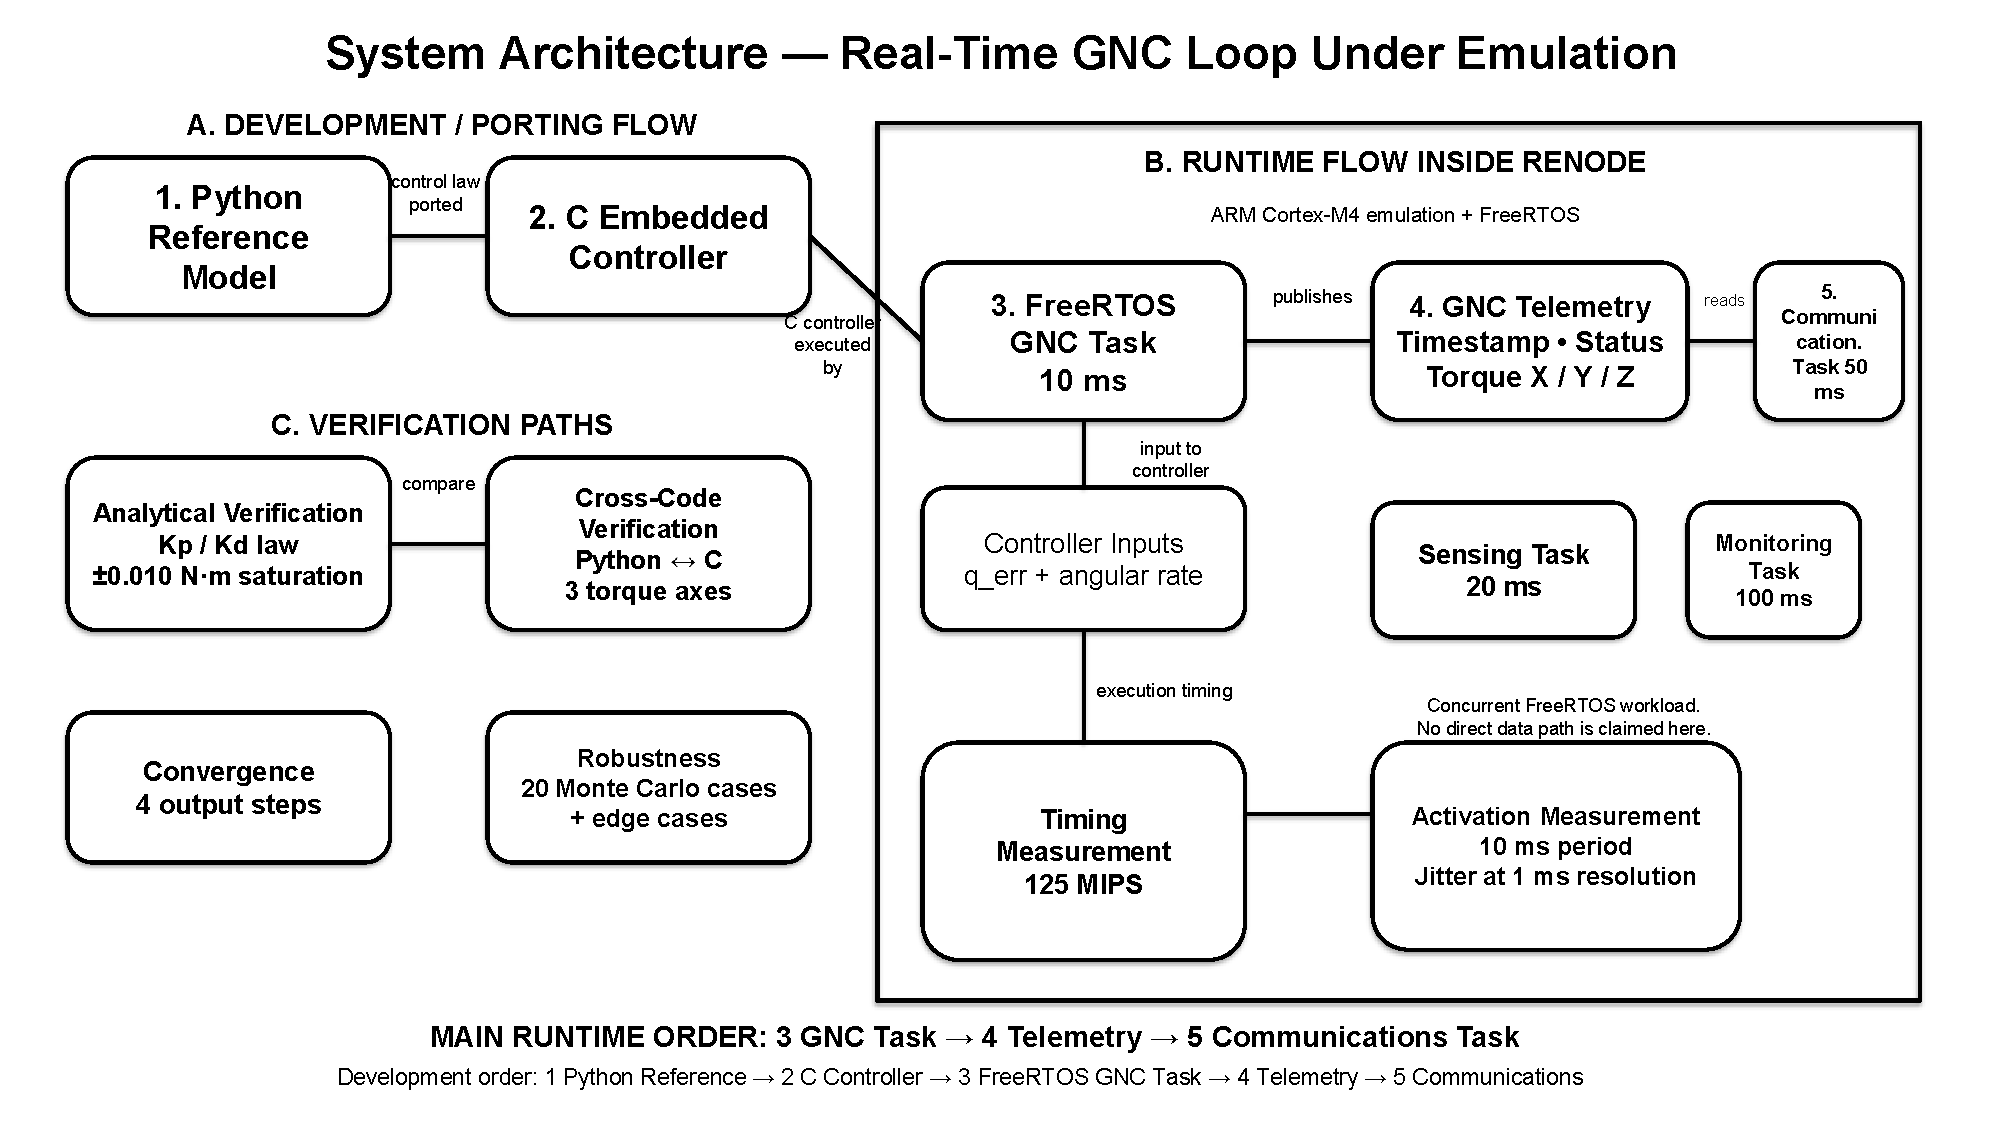
\includegraphics[width=\textwidth]{system_architecture_final.pdf}
\caption{Verified system architecture and data flow from the Python reference model to the embedded C controller, FreeRTOS GNC task, telemetry interface, and communications task. Sensing and monitoring are shown as concurrent workload without an asserted direct data path.}
\label{fig:system-architecture}
\end{figure}


\subsection{FreeRTOS Task Structure}

The real-time application separates the main activities into four tasks. The GNC task executes the controller and publishes its telemetry. The sensing task represents sensor-side processing, the communications task consumes the published GNC telemetry, and the monitoring task provides a lower-rate supervisory function. The verified task periods are 10 ms for GNC, 20 ms for sensing, 50 ms for communications, and 100 ms for monitoring.

Static task allocation and a 1 kHz FreeRTOS tick were used in the verified configuration. The GNC task was assigned the highest application priority among these tasks, followed by sensing, communications, and monitoring. This structure provides concurrent workload around the controller rather than measuring the controller only as an isolated function. The verified task relationships and scheduling context are summarized in Figure~\ref{fig:freertos-task-architecture}.

\begin{figure}[H]
\centering
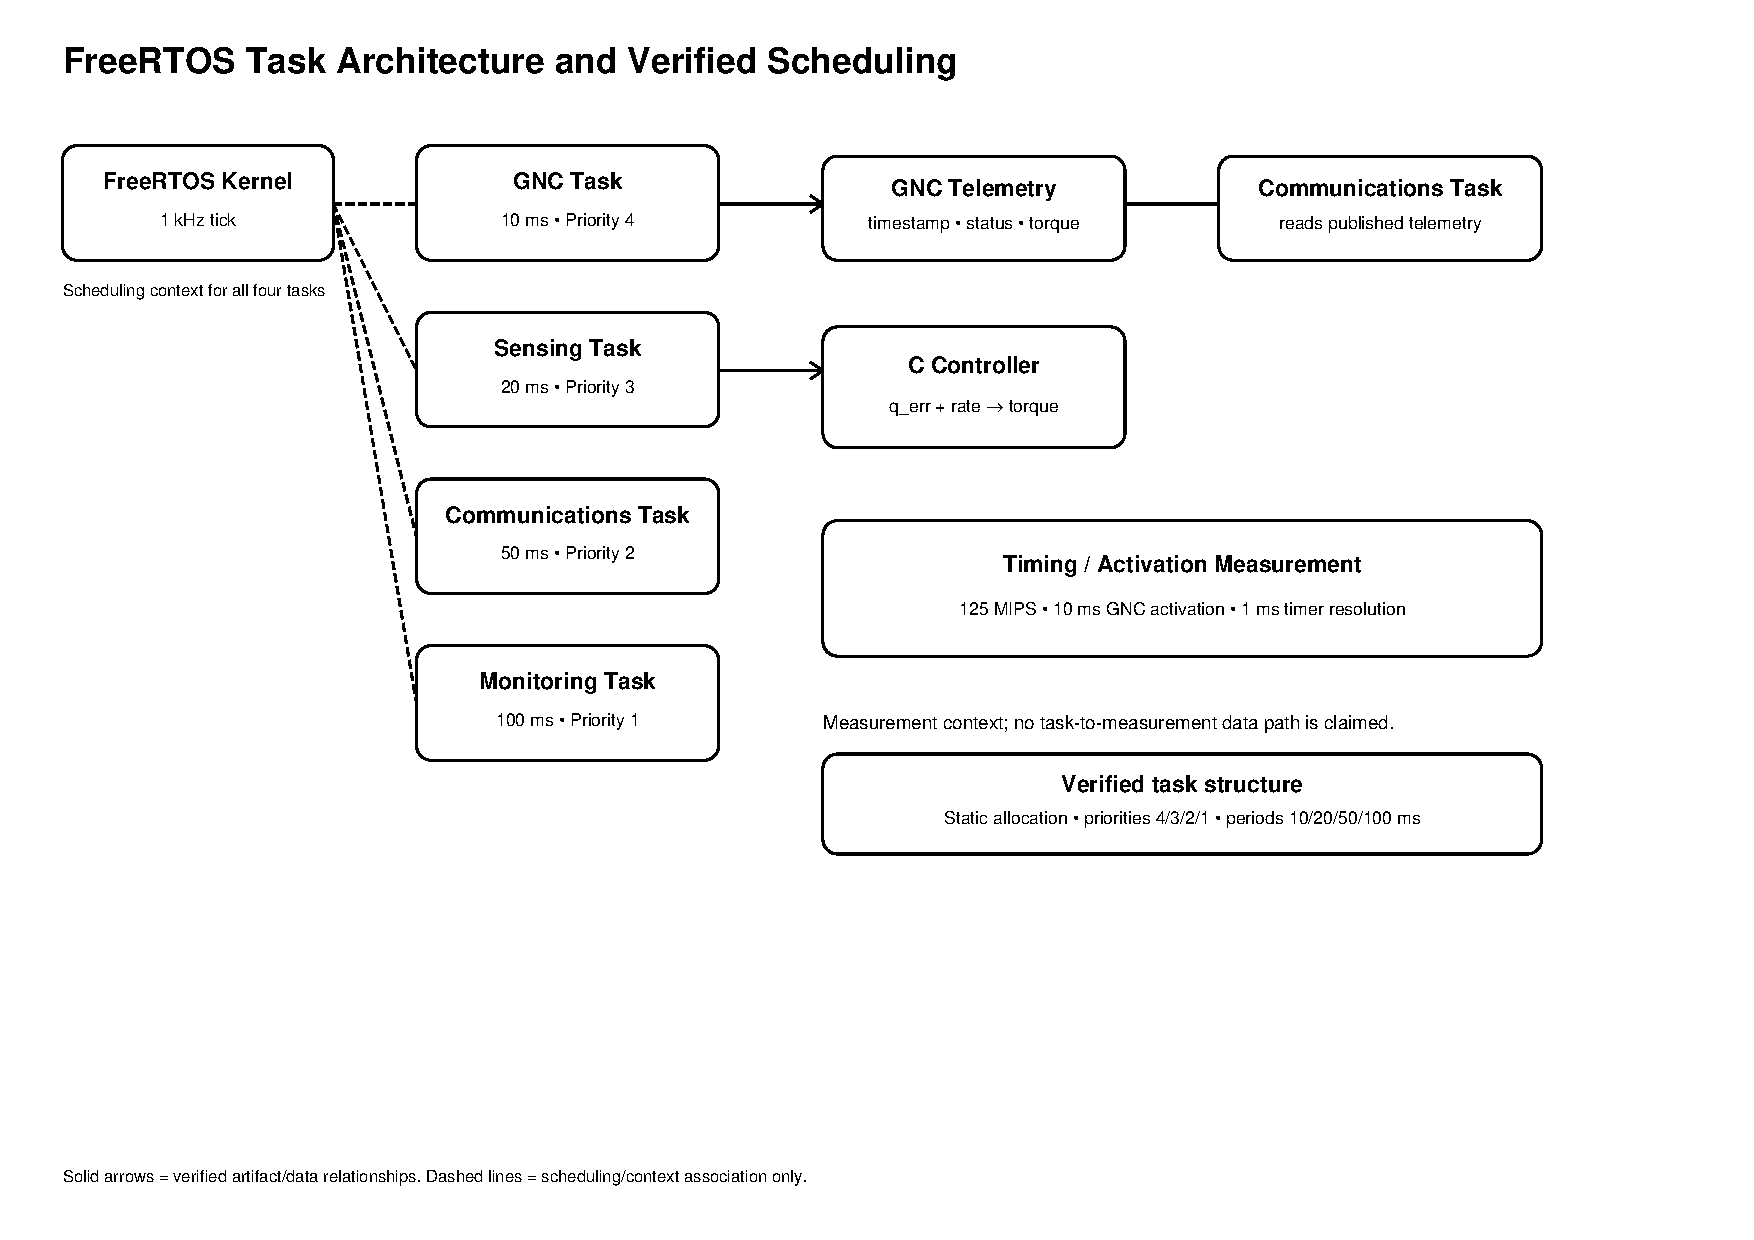
\includegraphics[width=\textwidth]{freertos_task_architecture.pdf}
\caption{Verified FreeRTOS task architecture showing the 1 kHz scheduling context, task periods and priorities, the GNC controller and telemetry path to Communications, and the timing-measurement context. Dashed lines indicate scheduling/context association rather than data flow.}
\label{fig:freertos-task-architecture}
\end{figure}

\subsection{Embedded Controller Artifact}

The embedded controller is implemented in C and is linked into the Cortex-M4 application. The controller output is retained in a telemetry structure containing a timestamp, status field, and three torque values. This interface became the real software artifact exchanged between the GNC-control side and the embedded-software/RTOS side during the Week 9 integration activity.


\section{Timing and Real-Time Measurements}

\subsection{Controller Execution-Time Measurement}

A dedicated controller benchmark was used to measure execution behaviour under the 125 MIPS emulated target configuration. Three representative controller cases were exercised: an unsaturated case, a positive saturation case, and a negative saturation case. The measured instruction counts correspond to 7.288 microseconds, 6.016 microseconds, and 5.968 microseconds, respectively.

The maximum observed execution time was therefore 7.288 microseconds and the minimum observed value was 5.968 microseconds, giving an observed spread of 1.320 microseconds. These values are measurements from the executed benchmark cases and are not claimed as a formal worst-case execution-time proof.

\subsection{Deadline Margin}

For a 10 ms GNC activation period, using the maximum observed controller execution time gives the observed timing margin:

\begin{equation}
T_{\mathrm{margin}}=10\ {\rm ms}-0.007288\ {\rm ms}=9.992712\ {\rm ms}.
\end{equation}

The large positive margin indicates that the measured controller execution occupies only a small fraction of the available 10 ms control period. The result remains qualified because the benchmark does not establish a formal WCET bound over every possible processor state, compiler path, interrupt condition, or future software configuration.


\subsection{Periodic Activation and Jitter}

The Week 11 final measurement recorded 100 GNC activations. The measured minimum and maximum activation intervals were both 10 timer ticks. With the configured 1 kHz FreeRTOS tick, this corresponds to a nominal 10 ms activation period.

The measured peak-to-peak jitter was 0 timer ticks, corresponding to 0 ms at the available 1 ms timer resolution. This result must not be interpreted as proof of zero sub-millisecond jitter. The measurement resolution is limited by the timer tick, so variations smaller than one tick are not observable in this experiment.

The execution-time tick fields in the Week 11 measurement were also zero because the controller completed within the same timer tick. They are therefore not converted to zero microseconds. The dedicated instruction-count benchmark remains the appropriate evidence for the controller execution-time measurement.

\subsection{Earlier Extended Timing Observation}

An earlier extended RTOS trace contained 12 controller intervals, each represented by 1025 timing records. These corresponded to approximately 8.20 microseconds per observed controller interval with zero observed spread in that trace. This result is retained as an additional observation from the RTOS-integrated environment, while the later dedicated benchmark provides the 7.288 microsecond maximum observed controller execution value used for the timing-margin calculation.


\section{Week 9 Cross-Domain Integration}

\subsection{Real Artifact Exchange}

The Week 9 integration exchanged a real software artifact between the Aerospace GNC control-model side and the Embedded Software/RTOS side. The exchanged artifact was the proportional-derivative control law together with its torque output interface. The Python-side control behaviour was represented by the embedded C controller, while the RTOS application exposed the resulting values through a GNC telemetry structure.

The telemetry interface contains a timestamp, status field, and three torque values. The GNC task updates this structure, while the Communications task reads the published telemetry. The interface therefore represents an actual producer-consumer exchange rather than a documentation-only connection.

\subsection{Cross-Code Numerical Verification}

A dedicated cross-code test used the same deterministic input as the analytical verification. The Python/reference result was [-0.010000, 0.007000, -0.003300] N m after saturation. The embedded C implementation produced exactly the same three values when represented in integer micro-torque units: -10000, 7000, and -3300 micro-units.

The three axes therefore agree exactly for the tested input. The test also verified completion through the test_done flag. Integer micro-units were used because the Renode memory inspection available during this test did not provide direct double-precision value reading. This is a measurement-interface limitation, not a numerical mismatch.

\subsection{Runtime Integration Evidence}

During Renode execution, the Communications task observed nonzero GNC timestamps and a status value of 1. The GNC counter also advanced substantially during the run. These observations verify that the GNC producer was executing and that the Communications consumer was reading updated telemetry.

The integration is therefore classified as \textbf{verified with qualification}. The software artifact exchange and numerical cross-code result are directly verified. The qualification is that the project does not contain a separate external partner-domain repository; the two sides are the Aerospace GNC reference/control model and the Embedded Software/RTOS implementation developed within this project.


\section{Convergence and Robustness Verification}

\subsection{Numerical Convergence}

The reference implementation was evaluated with output steps of 1, 0.5, 0.25, and 0.125 s. The final roll value was approximately -0.00000052 degrees for all four cases, while final pitch and yaw remained approximately zero. The maximum difference between consecutive reported final-attitude results was zero at the available output precision.

This result provides evidence that the reported final attitude is insensitive to the tested output-step values. It is nevertheless qualified because the underlying integration uses an adaptive RK45 method; identical sampled outputs do not independently establish convergence of the internal adaptive integration error.

\subsection{Gain Sensitivity}

The proportional-gain sensitivity study varied Kp while retaining Kd = 0.05. For Kp values of 0.004, 0.006, 0.008, 0.010, and 0.012, the reported final attitude error was 0.007471, 0.000087, 0.000001, 0, and 0 degrees, respectively. The corresponding saturation percentages were 0.94, 1.37, 1.77, 2.16, and 2.55 percent.

The derivative-gain study retained Kp = 0.008 and varied Kd over 0.025, 0.0375, 0.05, 0.0625, and 0.075. The final attitude errors were approximately 0.000001, 0.000001, 0.000001, 0.000042, and 0.000486 degrees, with saturation percentages of 2.93, 2.21, 1.77, 1.48, and 1.26 percent, respectively.

These results show a stable region around the selected nominal gains for the tested scenarios, while also demonstrating that changes in gain affect actuator saturation and transient behaviour.

\subsection{Monte Carlo Verification}

A 20-case Monte Carlo study using fixed random seed 42 was performed to examine sensitivity to perturbed initial conditions. The mean final attitude error was 0.000036 degrees and the maximum was 0.000543 degrees. The mean final angular-rate error was approximately 0.000002 deg/s, with a maximum of 0.000029 deg/s. The maximum observed saturation across the cases was 3.01 percent.

The fixed seed makes the experiment reproducible and allows the reported statistics to be regenerated from the same test configuration.

\subsection{Edge Cases}

Three representative edge cases were also evaluated. A 0 degree case produced zero final attitude error and zero final rate error with zero saturation. A 0.1 degree case produced approximately 0.000002 degrees final attitude error, approximately 0.000002 deg/s final rate error, and 0.01 percent saturation. A 90 degree case produced approximately 0.000002 degrees final attitude error, approximately zero final rate error, and 4.97 percent saturation.

The edge-case results support correct behaviour across small-error and large-angle test conditions within the tested configuration. They do not constitute a global stability proof.


\section{Published Reference Comparison}

\subsection{Selected Published Result}

A NASA-hosted thesis titled \textit{Attitude Determination \& Control System Design and Implementation for a 6U CubeSat Proximity Operations Mission} by Francisco J. Franquiz was selected as the published reference\cite{franquiz}. The thesis reports target-tracking performance for several attitude-control configurations. In Table 5.19, the scheduled-gain PID configuration reports a mean pointing accuracy of 0.35 arcmin for the Rate Observer case.

The published work also documents the target-tracking simulation setup, including an initial attitude and angular-rate condition, a 500 km orbit altitude, a 28.5 degree inclination, a 250 km distance to the reference spacecraft, a 10 Hz RCS thruster frequency, a 10 s gain-schedule transient, and a 1 ms simulation timestep. These details provide contextual information for comparison, but they do not provide the original numerical target-tracking time series required for exact numerical reproduction.

\subsection{Figure Digitization and Qualified Comparison}

Figure 5.4 of the published thesis was digitized to obtain an approximate representation of the plotted mean pointing-error curve. The digitized curve contained 735 extracted points over the plotted time interval. Its calculated mean was 0.3911 arcmin, compared with the published 0.35 arcmin benchmark.

The absolute difference is 0.0411 arcmin and the relative difference with respect to the published benchmark is approximately 11.74 percent. Because the source numerical time series was unavailable, the digitized curve cannot be treated as the original simulation data. The result is therefore classified as partial/qualified published-data verification rather than a full reproduction of the published simulation.



\begin{figure}[H]
\centering
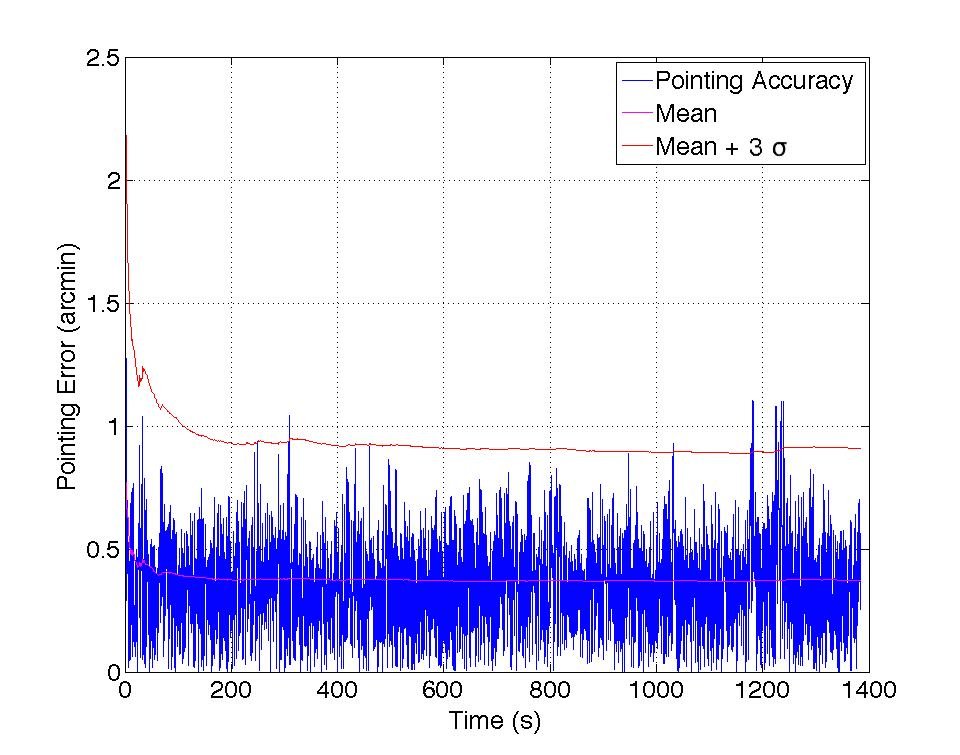
\includegraphics[width=0.85\textwidth]{figure_5_4.png}
\caption{Digitized representation of the published target-tracking pointing-error curve from Figure 5.4. The plot is used for qualified quantitative comparison and is not treated as the original numerical dataset.}
\label{fig:published-pointing-error}
\end{figure}
This distinction is important to the verification claim: the published benchmark was independently identified and the plotted result was quantitatively examined, but the unavailable original time series prevents a defensible claim that the present model reproduces the published numerical trajectory.


\section{Four-Way Verification Summary}

The project verification campaign combines four complementary evidence paths: analytical limits, published-data comparison, cross-code verification, and numerical convergence\cite{assignment}. The purpose is to avoid relying on a single successful execution result.

\subsection{Verification Evidence Counts}

Table~\ref{tab:verification-evidence} summarizes the principal executed verification cases. The entries report the available evidence without converting every execution into a generic unit-test pass claim.

\begin{table}[H]
\centering
\caption{Verification evidence and executed case counts}
\label{tab:verification-evidence}
\begin{tabular}{p{0.38\textwidth}p{0.18\textwidth}p{0.34\textwidth}}
\toprule
Verification evidence & Cases/items & Recorded result \\
\midrule
Deterministic analytical/controller test & 1 & Verified controller output and saturation \\
Cross-code torque comparison & 3 axes & Exact agreement \\
Numerical convergence & 4 output steps & Same final attitude at reported precision \\
Monte Carlo robustness & 20 cases & Executed; results within reported ranges \\
Edge-case analysis & 3 cases & Executed; results recorded \\
\bottomrule
\end{tabular}
\end{table}

\subsection{Verification Status}

\textbf{1. Analytical limits -- VERIFIED.} The controller torque calculation and actuator saturation were checked against the analytical bound. For the deterministic test case, the raw first-axis torque of -0.014 N m was correctly limited to -0.010 N m, while the other two axes remained at +0.007 N m and -0.0033 N m.

\textbf{2. Published data -- PARTIAL/QUALIFIED.} The published 0.35 arcmin benchmark was identified and Figure 5.4 was digitized. The digitized mean was 0.3911 arcmin, giving a 0.0411 arcmin absolute difference and an 11.74 percent relative difference. The original numerical time series was unavailable, so full reproduction is not claimed.

\textbf{3. Cross-code verification -- VERIFIED.} The deterministic Python/reference controller output and the embedded C controller output agreed exactly on all three axes. The C result was inspected using integer micro-torque units because direct double-precision memory reading was unavailable in the Renode inspection method.

\textbf{4. Numerical convergence -- VERIFIED WITH QUALIFICATION.} The tested output steps of 1, 0.5, 0.25, and 0.125 s produced the same reported final attitude at the available output precision. This supports output-level convergence for the tested cases, but does not by itself prove convergence of the internal adaptive RK45 integration error.

\subsection{Overall Assessment}

Three verification paths are directly supported by project evidence, while the published-reference path remains partial and qualified. The overall result is therefore not classified as complete four-way reproduction. Instead, the evidence demonstrates verified analytical behaviour, exact cross-code agreement, qualified numerical convergence, and a quantitatively examined but incomplete published-reference comparison.


\section{Failures, Limitations, and Negative Results}

\subsection{Initial Timing Failure}

The first timing experiment did not produce a defensible execution-time result. The benchmark terminated with an ARM UsageFault associated with an INVSTATE condition, with the program counter reported as 0xFFFFFFFE and the CFSR value reported as 0x00020000. Because the timing run did not complete correctly, its result was excluded from the timing claims. A separate benchmark was subsequently constructed and executed successfully.

\subsection{Measurement Resolution Limitation}

The Week 11 jitter measurement used a 1 ms timer resolution. The observed peak-to-peak jitter was zero timer ticks, but this does not establish zero jitter below the timer resolution. Similarly, execution-time tick counters that remained within one timer tick were not interpreted as zero microseconds. The dedicated instruction-count benchmark was used instead for the controller execution-time result.

\subsection{Published-Data Reproduction Limitation}

The published-reference experiment could not be reproduced from the original numerical data because the thesis did not provide the numerical target-tracking time series used to generate the relevant plot. Figure digitization was therefore used only as a qualified comparison. The 0.3911 arcmin digitized mean should not be presented as the original published numerical dataset.

\subsection{Reproducibility Limitation}

The project contains a clean relative-path reproduction script for the Week 9 integration. However, several legacy Renode scripts retain machine-specific absolute paths. A project-wide clone-and-run reproduction without modification is therefore not claimed. This limitation is explicitly documented rather than silently changing the verified legacy scripts.

\subsection{Scope of the Verification}

The project demonstrates functional agreement, timing observations, integration behaviour, robustness testing, and several independent verification paths. It does not establish a formal mathematical global-stability proof, a formal WCET bound, or complete reproduction of the published target-tracking simulation. These remain appropriate areas for future work.


\section{Reproducibility and Repository}

Reproducibility was treated as a project requirement rather than only a documentation task. The final project directory contains the source code, embedded artifacts, verification scripts, evidence files, and a README describing the execution environment and major reproduction paths.

\subsection{Execution Environment}

The verified environment used Python 3.12.3 with NumPy 2.5.0 and SciPy 1.18.1 for the reference simulation\cite{python,scipy}. The embedded target was an ARM Cortex-M4 environment using arm-none-eabi-gcc 15.3.1\cite{arm_m4_trm,arm_m4_data}. Renode 1.17.0 was used for emulation with a configured performance rate of 125 MIPS\cite{renode_time,renode_exec,renode_metrics}. FreeRTOS was used for the real-time task architecture\cite{freertos_task,freertos_manual}.

\subsection{Repository Structure and Evidence}

The project repository contains the Python reference model, C controller implementation, FreeRTOS integration, Renode scripts, timing and robustness scripts, analytical verification outputs, cross-code verification evidence, published-reference comparison material, and the project README. Large generated traces and the downloaded published PDF were excluded from the Git repository where appropriate.

\subsection{Reproduction Paths}

The Week 9 integration has a relative-path Renode reproduction script that loads the corresponding ELF from the working directory. The cross-code verification can be reproduced from the deterministic input case and compares the embedded controller output with the Python/reference result. The README records the principal tools, versions, evidence files, and interpretation of the timing measurements.

\subsection{Version Control}

The completed implementation and verification artifacts were committed to Git and pushed to the project repository at \url{https://github.com/rakshitalb/VESPER-Real-time-GNC}. The repository therefore provides a shared version-controlled record of the submitted implementation and supporting evidence.

\subsection{Remaining Reproducibility Gap}

Although the main evidence is preserved and the Week 9 reproduction path is clean, the project is not claimed to be fully clone-and-run reproducible because legacy Renode scripts contain machine-specific absolute paths. This is recorded as a known limitation rather than hidden through unverified modifications.


\section{Recommendations and Future Work}

The completed verification campaign identifies several improvements that would strengthen the system beyond the present scope.

\subsection{Higher-Resolution Timing Measurement}

A cycle counter or instruction-level hardware performance counter should be used in a future implementation to measure controller execution time and jitter below the 1 ms timer resolution. This would provide a stronger timing characterization than the current tick-based periodic measurement.

\subsection{Formal WCET Analysis}

The present execution-time result is a maximum observed measurement rather than a formal worst-case execution-time bound. Future work should combine measured traces with static timing analysis or a sufficiently justified exhaustive path analysis to establish a defensible WCET bound.

\subsection{Complete Published-Result Reproduction}

A complete reproduction of the published target-tracking result would require the original numerical reference trajectory or sufficient information to reconstruct it exactly. If the original dataset becomes available, the present digitization workflow should be replaced by direct numerical comparison using the published time series.

\subsection{Expanded Cross-Domain Integration}

The current Week 9 exchange demonstrates a real artifact interface between the aerospace GNC model and embedded software implementation\cite{assignment}. Future work should extend this exchange to an independently maintained adjacent-domain artifact, such as a fitted plant parameter set, navigation measurement dataset, or hardware-in-the-loop interface.

\subsection{Automated Verification}

Future revisions should introduce a conventional automated test framework with an explicit pass/fail count covering controller equations, saturation, numerical reference agreement, interface serialization, and regression cases. The present project intentionally does not claim a conventional unit-test suite because the existing evidence was produced through dedicated verification scripts and runtime measurements.

\subsection{Hardware Validation}

The current implementation is validated through compilation and Cortex-M4 emulation\cite{arm_m4_trm,renode_exec}. A further stage would deploy the controller on physical Cortex-M4 hardware and compare measured execution time, task scheduling, sensor-interface behaviour, and actuator-command timing against the Renode results.


\section{Consolidated Results}

Table~\ref{tab:baseline-results} summarizes the principal quantitative results obtained during the reference simulation, embedded implementation, timing study, and robustness campaign.

\begin{table}[H]
\centering
\caption{Principal quantitative results}
\label{tab:baseline-results}
\begin{tabular}{p{0.43\textwidth}p{0.22\textwidth}p{0.25\textwidth}}
\toprule
Metric & Result & Verification status \\
\midrule
Deterministic C/Python torque comparison & -0.0100, +0.0070, -0.0033 N m & Exact agreement \\
Maximum observed controller execution time & 7.288 microseconds & Measured observation \\
Minimum observed controller execution time & 5.968 microseconds & Measured observation \\
Execution-time spread & 1.320 microseconds & Measured observation \\
Control-period deadline & 10 ms & Defined requirement \\
Deadline margin & 9.992712 ms & Calculated \\
Periodic activation period & 10 ms & Measured \\
Observed jitter at 1 ms resolution & 0 ms p-p & Qualified measurement \\
Published benchmark & 0.35 arcmin & Source result \\
Digitized published-figure mean & 0.3911 arcmin & Qualified comparison \\
\bottomrule
\end{tabular}
\end{table}

\subsection{Reference Scenario Results}

\begin{table}[H]
\centering
\caption{Recorded reference simulation scenarios}
\label{tab:scenario-results}
\begin{tabular}{p{0.30\textwidth}p{0.27\textwidth}p{0.25\textwidth}}
\toprule
Scenario & Main result & Saturation \\
\midrule
Free drift, 600 s & Final angular rate magnitude 0.0436 deg/s; final roll -31.479 deg & 0 percent \\
30 deg rest-to-rest PD, 200 s & Final attitude approximately zero & 1.8 percent \\
30 deg rest-to-rest LQR, 200 s & Final attitude approximately zero & 14.3 percent \\
45 deg yaw slew PD, 300 s & Final yaw -45 deg & 3.1 percent \\
45 deg yaw slew LQR, 300 s & Final yaw -45 deg & 20.0 percent \\
\bottomrule
\end{tabular}
\end{table}

\subsection{Interpretation}

The consolidated results show that functional correctness and real-time execution were evaluated separately. The controller output was checked directly against the analytical reference, while execution timing was measured using dedicated embedded benchmarks. The published comparison was kept separate because its source data were incomplete. This separation prevents a successful result in one verification route from being incorrectly used as evidence for another.

\section{Conclusions}

This work developed and verified a real-time spacecraft attitude-control loop under Cortex-M4 emulation. The workflow connected a Python reference model to an embedded C implementation, integrated the controller with a FreeRTOS task structure, and executed the resulting software in Renode.

The verification campaign produced several independently supported results. The deterministic controller case showed exact agreement between the Python/reference implementation and the embedded C implementation on all three torque axes. Analytical checks confirmed the controller law and actuator saturation behaviour. Timing measurements established a maximum observed standalone controller execution time of 7.288 microseconds, corresponding to a 9.992712 ms margin against the 10 ms control period. The periodic activation measurement showed a 10 ms period with zero observed peak-to-peak jitter at the 1 ms timer resolution.

The numerical reference model was also subjected to convergence, gain-sensitivity, Monte Carlo, and edge-case analysis. These tests showed consistent behaviour for the tested parameter ranges and scenarios. The Week 9 integration further demonstrated exchange of a real control artifact between the aerospace GNC model and embedded real-time software through the C controller and telemetry interface.

The published-reference comparison was intentionally reported with a qualification. A published 0.35 arcmin target-tracking benchmark was identified, and Figure 5.4 was digitized to obtain an approximate mean of 0.3911 arcmin. Because the original numerical time series was unavailable, this result does not constitute full reproduction of the published simulation. Likewise, the measured 7.288 microsecond execution time is a maximum observed value rather than a formal WCET bound.

Overall, the project demonstrates a reproducible and evidence-driven workflow for connecting spacecraft GNC simulation with embedded real-time execution. The strongest results are the exact cross-code verification, analytical actuator-limit verification, real-time integration evidence, and quantified timing measurements. The remaining limitations are explicitly documented and provide a clear basis for future higher-resolution timing analysis, formal WCET analysis, complete published-result reproduction, automated testing, and physical hardware validation.


\begin{thebibliography}{18}

\bibitem{assignment} EduRankAI, ``VISVAMBHARA -- Weeks 4--12 Remote Task Assignment VESPER-TASK-W412-002'' 2026.

\bibitem{renode_time} Renode, ``Time framework'' Renode Documentation.

\bibitem{renode_exec} Renode, ``Basic execution control'' Renode Documentation.



\bibitem{renode_metrics} Renode, ``Execution metrics, profiling and opcode counting'' Renode Documentation.


\bibitem{arm_m4_trm} Arm, ``Arm Cortex-M4 Processor Technical Reference Manual'' Arm Developer.

\bibitem{arm_m4_data} Arm, ``Arm Cortex-M4 Processor Datasheet'' Arm Developer.



\bibitem{freertos_task} FreeRTOS, ``Implementing a Task'' FreeRTOS Documentation.

\bibitem{freertos_manual} FreeRTOS, ``FreeRTOS Reference Manual'' FreeRTOS.

\bibitem{python} Python Software Foundation, ``Python 3 Documentation.''

\bibitem{scipy} SciPy Community, ``solve_ivp -- SciPy API Reference.''


\bibitem{franquiz} F. J. Franquiz, ``Attitude Determination \& Control System Design and Implementation for a 6U CubeSat Proximity Operations Mission'' NASA-hosted thesis.


\end{thebibliography}


\end{document}






